
%% brief overview of how the the results are organized

We present our results in four parts. First, we provide correlational evidence for the three propositions derived from our model. We then discuss alternative explanations and how we deal with them. Third, we present various additional robustness analyses. Lastly, we explore which firms are more likely to launch multiple experiments, and which firms try novel approaches.

%%-------------------------------------------------------------
%%
%%
%%
%% [SUBSECTION] BASELINE CORRELATIONAL RESULTS
%%
%%
%%
%%-------------------------------------------------------------

\subsection{Diversity of Approaches and the Success of Experimentation}


We begin by examining, correlationally, the relationships theorized by Propositions 1 and 2 between experimenter scale, the diversity of approaches, and the average success of experimentation. We estimate the following econometric specification:


\begin{equation}
\label{eq:baseline_model}
\begin{aligned}
        y_{i, t} = \alpha + \beta_1{x_{i, t}} + \theta_{i, t} + \gamma_i\times\tau_t + \epsilon_{i, t}
\end{aligned}
\end{equation}

Where $y_{i, t}$ represents the market-year level dependent variable \emph{Target Diversity}, or \emph{Share of Pre-Clinical Success}. and $x_{i, t}$ is the average experimenter scale in a therapeutic class--year. We test this specification with and without $\theta_{i, t}$, which is our set of market structure control variables for the number of firms, targets, and pre-clinical experiments within a therapeutic class–year. In all models we include ATC-1$\times$Year fixed effects $\gamma_i\times\tau_t$, amd standard errors are clustered at the ATC-1 level to account for correlations in errors among market observations within the same industry group.

\begin{table}[h!]
    \centering
    \scriptsize
    \caption{\textsc{The market-level relationship between experimenter scale, the diversity of approaches, and success}}
    \vspace{1em}
        \input{tables/featured/all-props-baseline-correlations}

    \label{tab:baseline-regressions-all-props}
    \vspace{1em}
    \caption*{\scriptsize\emph{Notes:} This Table reports baseline regression results testing each Proposition. In columns (1) and (2), we test Proposition \ref{prop:model-choice} by regressing \emph{Target Diversity} on \emph{Average Experimenter Scale}, where the difference between the two models is that column (2) includes the set of \emph{Market Structure Controls}. \emph{Target Diversity} is the Shannon entropy of the relative abundance of targets employed in pre-clinical experiments, and \emph{Average Experimenter Scale} is the average number of pre-clinical experiments started by firms in a therapeutic class--year. In columns (3) and (4), we test Proposition \ref{prop:model-outcomes} by regressing the \emph{Share of Pre-Clinical Success} on \emph{Average Experimenter Scale}. Lastly, columns (5) and (6) correspond to Proposition \ref{prop:atleastone}, where we explore the relationship between \emph{Target Diversity} and \emph{At least 1 Pre-Clinical Success}. All models are estimated with OLS. Robust standard errors clustered at the ATC-1 level are shown in parentheses. Significance codes: * p<.1, ** p<.05, *** p<.01 }
\end{table}

We present the results from this baseline specification in Table \ref{tab:baseline-regressions-all-props}. Column (1) reports the baseline relationship between experimenter scale and target diversity, showing a positive and significant association. In column (2), we incorporate market structure controls. Notably, the estimated coefficient for $\beta_1$ remains consistent across models. Based on the estimate in column (2), our findings suggest that a 1-unit increase in the average experimenter scale (e.g., from an average of 1.1 to 2.1 experiments per firm) corresponds to a 1.65 standard deviation increase in target diversity, which is consistent with Proposition \ref{prop:model-choice}.

In columns (3) and (4) we test Proposition \ref{prop:model-outcomes}: small-scale experimenters are more likely to be successful in an individual experiment than large-scale experimenters. Here we regress the \emph{Share of Pre-Clinical Success} on \emph{Average Experimenter Scale}, and find a negative relationship, consistent with our prediction. 

Lastly, to test Proposition \ref{prop:atleastone} we estimate the specification detailed in Equation \ref{eq:baseline_model} where the independent variable $x_{i, t}$ is \emph{Target Diversity} and the dependent variable $y_{i, t}$ is \emph{At least 1 Pre-Clinical Success}. The results are presented in columns (5) and (6) of Table \ref{tab:baseline-regressions-all-props}. Consistent with Proposition \ref{prop:atleastone}, these results indicate that markets with greater approach diversity in experimentation have a higher probability of at least one success. 


\begin{figure}[h!]
\caption{\textsc{Binned scatter plots of the market-level relationship between experimenter scale, the diversity of approaches, and success}}
\label{fig:baseline-nonparametrics}
    \centering
    \begin{subfigure}[t]{.3\textwidth}
        \centering
        \caption{Target Diversity}
        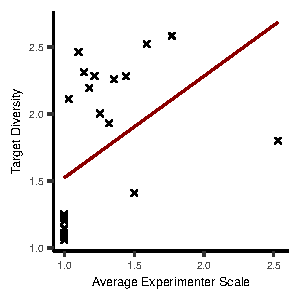
\includegraphics[width=\linewidth]{figures/featured/target_diversity_exp_scale.pdf}
    \end{subfigure}
    \begin{subfigure}[t]{.3\textwidth}
        \centering
        \caption{Average Success}
        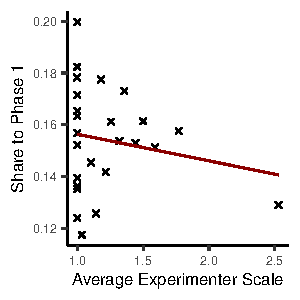
\includegraphics[width=\linewidth]{figures/featured/scale_phase1_share.pdf}
    \end{subfigure}
        \begin{subfigure}[t]{.3\textwidth}
        \centering
        \caption{At least one success}
        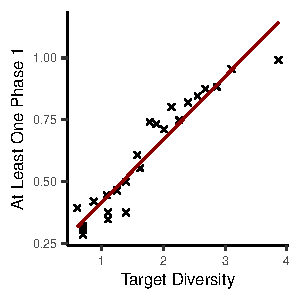
\includegraphics[width=\linewidth]{figures/featured/diversity_atleastone_phase1.pdf}
    \end{subfigure}
\caption*{\scriptsize\emph{Notes:} This Figure shows non-parametric binned scatter plots of the relationship between \emph{Target Diversity}, \emph{Average Experimenter Scale}, the \emph{Share of Pre-Clinical Success}, and \emph{At least 1 Pre-Clinical}, corresponding to the parametric estimates in Table \ref{tab:baseline-regressions-all-props}. Each plot uses 25 bins. }
\end{figure}

%%-------------------------------------------------------------
%%
%%
%%
%% [SUBSECTION] ALTERNATIVE EXPLANATIONS
%%
%%
%%
%%-------------------------------------------------------------
\subsection{Alternative Explanations}

Establishing causality in this context is challenging. The ideal experiment would involve identifying a source of exogenous variation in the cost or value of experimentation for certain firms in a market. For instance, a reduction in the cost of experimentation for some firms within a market could lead to an increase in the number of experiments they initiate, thereby altering the average experimenter scale without directly affecting the diversity of approaches used. While shocks that influence entire markets do exist---for example, the introduction of Medicare Part D in 2004, which arguably increased the value of experimentation in therapeutic classes with predominantly elderly patients \citep{dranove2022does}---such shocks tend to affect \emph{all} firms operating in the market.\footnote{One possible refinement could consider the geographic dimension of drug development. Since Medicare Part D was enacted in the U.S., its impact may have been limited to U.S. pharmaceutical firms within relevant therapeutic classes. However, because pharmaceutical companies operate globally, they are unlikely to be geographically isolated. Moreover, a shock like Medicare Part D could produce mixed effects. While it might encourage firms previously conducting only one experiment to initiate two, it could also incentivize new market entry, enabling firms that otherwise would not have participated to conduct experiments. Consequently, the impact on the composition of the experimenter scale within a market remains ambiguous.}

Instead, we take a multipronged approach to evaluate alternative explanations that would undermine our results. Our strongest argument is that neither alternative explanations nor likely sources of unobserved heterogeneity can explain the pattern of empirical results regarding the success of experimentation (Propositions \ref{prop:model-outcomes} and \ref{prop:atleastone}):  that greater experimenter scale increases the probability of at least one success but lowers average success. If the relationship between the average experimenter scale and target diversity were driven solely by unobserved common variables, we would not expect higher target diversity to correlate with both a higher probability of at least one success and a lower average share of successes in the market. 

For instance, suppose that some markets have more technical opportunities, and this is positively (negatively) associated with the number of approaches observed. Then, there should be a positive (negative) relationship between diversity and average success but also at least one success. There is no reason to expect a relationship between diversity and average size. Alternatively, suppose, for some reason, experimenter-scale is positively related to technological opportunity, which, in turn, is positively related to the diversity of approaches. This would result in a positive association between experimenter-scale and diversity. However, this should also increase, not decrease, average success. Thus, while we cannot establish a causal link between experimenter scale and target diversity, the observed associations between experimenter scale, target diversity, and success outcomes are consistent with the hypothesized causal relationship.

\begin{table}[h!]
    \centering
    \scriptsize
    \caption{\textsc{Linking approach diversity to the success of experiments}}
    \label{tab:linking-diversity-to-success}
    \vspace{1em}
        \input{tables/featured/link-diversity-to-success}
    \vspace{1em}
    \caption*{\scriptsize\emph{Notes:} This Table reports regression results that link success outcomes to the diversity of targets, while controlling for the average scale of experimenters in the market. In column (1), we regress \emph{Share of Pre-Clinical Success} on  \emph{Target Diversity}, and in column (2) we include \emph{Average Experimenter Scale} as a control. Columns (3) and (4) are similar, but the dependent variable is \emph{At least 1 Pre-Clinical Success}. All models are estimated with OLS. Robust standard errors clustered at the ATC-1 level are shown in parentheses. Significance codes: * p<.1, ** p<.05, *** p<.01 }
\end{table}


%%--- other controls
There are some possible confounding variables which we can observe and directly control for. The first concerns the discovery of new targets. Our model and simulations assume a fixed pool of approaches from which firms select for experimentation, but the landscape of available approaches may evolve over time. The discovery of new targets and their relationships with therapeutic indications could expand the pool of available approaches, naturally increasing target diversity. Additionally, this dynamic could influence the composition of experimenter scale in the market if single- or multi-experiment firms differ in their likelihood of introducing novel targets.

Second, there could be underlying average firm characteristics within a market that are correlated with both the number of experiments firms' choose to launch and their choice of approach. For instance, younger firms may be less likely to conduct multiple experiments due to limited resources to fund and manage them. Additionally, if younger firms are more inclined to pursue novel approaches, the average firm age in a market could be correlated with target diversity.

In Table \ref{tab:all-props-baseline-with-controls}, we replicate the analysis from Table \ref{tab:baseline-regressions-all-props}, adding controls for discovery and average firm age. In column (1), the coefficient on \emph{Average Experimenter Scale} increases in magnitude when $\ln(Discovery)$ is included compared to the baseline result in column (1) of Table \ref{tab:baseline-regressions-all-props}, suggesting that the baseline model may underestimate the effect due to a downward bias. However, these results are limited by a smaller sample size, stemming from challenges in mapping new target discoveries to therapeutic classes. In column (2), which includes only the control for average firm age, the coefficient remains consistent with the baseline results reported in column (3) of Table \ref{tab:baseline-regressions-all-props}. Using the estimate from the full model in column (3), we find that a 1-unit increase in the average experimenter scale is associated with a 1.38 standard deviation increase in target diversity, slightly smaller than the baseline result.

As for the average success of experimentation, the inclusion of our control for discovery supresses the negative relationship reported between \emph{Average Experimenter Scale} and \emph{Target Diversity}. Still, after controlling for discovery we find no relationship between average exeperimenter scale and average success. Note that in column (5), which only includes the control for average firm age, the estimated coefficient is indistinguishable from the baseline estimate in column (4) of Table \ref{tab:baseline-regressions-all-props}.

Lastly, column (7) through (9) report the relationship between diversity and at least one pre-clinical success after controlling for target discovery and average firm age. When $\ln(Discovery)$ is included, the estimated coefficient on \emph{Target Diversity} is marginally less than the baseline result in column (6) of Table \ref{tab:baseline-regressions-all-props}. This suggests that the baseline model may slightly overestimate the effect due to a upward bias. Yet, we still find a positive and statistically significant relationship between the diversity of targets and the likelihood of at least one pre-clinical success.


\begin{table}[h!]
    \centering
    \scriptsize
    \caption{\textsc{The relationship between experimenter scale and target diversity while controlling for target discovery and firm age}}
    \vspace{1em}
    \resizebox{\textwidth}{!}{
        \input{tables/featured/all-props-baseline-with-controls}
    }
    \label{tab:all-props-baseline-with-controls}
    \vspace{1em}
    \caption*{\scriptsize\emph{Notes:} This Table reports baseline regression results testing each Proposition while controlling for two observable potential confounders. In columns (1) through (3), we regress \emph{Target Diversity} on \emph{Average Experimenter Scale}. Column (1) includes \emph{ln(Discovery)}, column (2) includes \emph{Average Firm Age}, and column (3) includes both variables. Recall that \emph{ln(Discovery)} is the natural logarithm of the count of publications in GWAS that report a novel target, and \emph{Average Firm Age} is the average age of distinct experimenters (firms) in a therapeutic class--year. The remaining models follow the same pattern, where the dependent variable in columns (4) through (6) is \emph{Share of Pre-Clinical Success}, and in columns (7) through (9) the dependent variable is \emph{At least 1 Pre-Clinical Success}. Note that in the final three columns---consistent with the baseline results in Table \ref{tab:baseline-regressions-all-props} that test Proposition \ref{prop:atleastone}---the indepednent variable of interest is  \emph{Target Diversity}. All models are estimated with OLS. Robust standard errors clustered at the ATC-1 level are shown in parentheses. Significance codes: * p<.1, ** p<.05, *** p<.01}
\end{table}



\begin{table}[h!]
    \centering
    \scriptsize
    \caption{\textsc{Alternative Explanations}}
    \label{tab:alternative-explanations}
    \vspace{1em}
        \input{tables/featured/alternative-explanations} 
    \vspace{1em}
\end{table}



\begin{comment}
refer to emily oster approach that considers size of coefficient change
\end{comment}



%%-------------------------------------------------------------
%%
%%
%%
%% [SUBSECTION] ROBUSTNESS
%%
%%
%%
%%-------------------------------------------------------------

\subsection{Robustness}

We also subject our baseline results to a series of robustness tests. The first addresses the complication that arise when a target is known to be a valid approach. In our model, this corresponds to an approach where $\pi$—the probability that the approach is a viable solution to the problem—equals one, meaning there is \emph{no} uncertainty about its viability. When $\pi=1$, the key implication is that outcomes for experiments using the same approach are no longer correlated, as success depends solely on implementation (see Appendix \ref{app:proofs}). In this case, firms will naturally select the approach with they have the highest probability of implementation success. We restrict the underlying project-level dataset to projects where the target chosen has not been successfully drugged, which we measure by the first launched product. In Appendix Table \ref{app:drop_pi_equal_one}, we replicate our core results in Table \ref{tab:baseline-regressions-all-props}, and find quantitatively similar estimates.

Second, we test the sensitivity of our results to alternate time windows. The unit of analysis in our baseline results is the therapeutic class--year. The choice to look within a single year is arbritary, so we construct two additional datasets, where we define observations within a two-year and five-year window. Table \ref{app:longer_time_windows} in the Appendix reports these results. Although we lose the number of observations through a higher level of aggregation, we find results consistent with our preferred specification which defines observations within a 1-year period. The only exception is that we lose statistical signficance between average experimenter scale and average success in the therapeutic class--five year period data, and find no relationship instead.

Third, we explore the robustness of our results to alternate measures of key variables. In particular, we test the sensitivity of our results to measuring target diversity with the Herfindahl-Hirschman Index. We also test an alternative measure to success, where we define success as whether a pre-clinical experiment ultimately results in a drug product launch. Table \ref{app:alternative_measures} in the Appendix shows results qualitatively similar to our baseline finding with these alternative measures.

Lastly, we attempt to address possible simultaneity bias by leveraging the panel structure of our data. Specifically, we use the average experimenter scale in the previous year $(i, t-1)$ as an instrument for the average experimenter scale in year $t$. This instrument relies on the assumption that idiosyncratic factors, unrelated to target diversity or underlying success probabilities, drive some markets to have more firms with lower experimentation costs. If these factors are persistent, the lagged experimenter scale would be correlated with the current experimenter scale but would not capture time-varying unobserved variables that influence experimenter-scale and target diversity.\footnote{Using the lagged experimenter scale as an instrument helps address simultaneity bias, but it cannot fully account for unobserved, market-specific and time-persistent factors---such as market dynamics, innovation strategies of firms, or public research funding across markets ---that may influence both experimenter scale and target diversity. However, our results are robust to controlling for aggregate industry-level time trends, captured by ATC-1$\times$Year fixed-effects  \citep{branstetter2022generic}.} We find, as described in Appendix Table \ref{app:2sls}, that the relationship between target diversity and experimenter-scale is strengthened.


%%-------------------------------------------------------------
%%
%%
%%
%% [SUBSECTION] WHICH FIRMS DO WHAT?
%%
%%
%%
%%-------------------------------------------------------------

\subsection{Which firms do multiple experiments and introduce novelty?}\label{subsec:which-firms}

Our data and results raise at least two questions, which we explore in this section. First, we have not addressed which firms choose to launch multiple experiments. One potential mechanism, demonstrated in our simulations, involves exogenously shifting the share of multi-experiment firms by altering the proportion of firms facing high or low experimentation costs. Alternatively, the same outcome could be achieved by allowing some firms to extract greater value from experiments, prompting them to enter with additional experiments.

A large body of research in Strategy and Economics suggests that firm size likely explains this pattern. Specifically, multi-experiment firms are most likely \emph{large}, as they benefit from lower experimentation costs \citep{cohen1996reprise} and can appropriate greater value from experiments \citep{arora2023invention}. This advantage stems, in part, from their complementary downstream co-specialized assets, which are essential for commercialization \citep[e.g.,][]{rosenbloom2000leadership, filippetti2017appropriability}.

We use firm ownership as a proxy for firm size, distinguishing between private and public firms. Interestingly, the data provide no evidence that public firms are more likely to conduct multiple experiments in a market. In panel (a) of Figure \ref{fig:firm-heterogeneity}, we show that private firms conduct only one experiment in a therapeutic class–year 61.5\% of the time. For public firms, this share is slightly \emph{higher}, at 63.3\%. Panel (b) presents the raw counts of experiments by experimenter scale. While public firms conduct significantly more experiments overall, the data reveal that, most of the time, they launch only one pre-clinical experiment in a therapeutic class–year.


Second, considering the discovery of new targets adds an intriguing nuance: which firms are more likely to introduce novelty? Specifically, when a new target–therapeutic class link is discovered, which firms—if any—are more likely to be the first to pursue this approach in pre-clinical trials? In panel (c) of Figure \ref{fig:firm-heterogeneity}, we plot the share of experiments by single-experiment firms and multi-experiment firms (those conducting more than one experiment in a therapeutic class–year) that are the first to use a target in a therapeutic class.

To ensure reliability, we include only projects initiated since 2005, as earlier projects are more likely to represent the first target–therapeutic class combinations due to the dataset’s starting point in 1995, which excludes targets drugged before this year. Panel (c) shows that single-experiment firms are more likely to drug a novel target: 54.9\% of experiments by these firms introduce a new target, compared to 45.9\% for multi-experiment firms. However, panel (d) reveals no significant difference between private and public firms in their likelihood of targeting a novel approach.

These results highlight a critical trade-off in the optimal allocation of experiments within a market. Markets dominated by small-scale experimenters are less favorable for innovation in some respects, as they are more likely to rely on a less diverse set of approaches and are less likely to achieve at least one successful experiment. However, these markets are also more likely to introduce new targets, drugging them for the first time.

\begin{figure}[h!]
\caption{\textsc{The relationships between ownership, experimenter scale, and the likelihood of experimenting with novel targets}}
\label{fig:firm-heterogeneity}
    \centering
    \begin{subfigure}[t]{.24\textwidth}
        \centering
        \caption{}
        \includegraphics[width=\linewidth]{figures/private_public_same_scale.pdf}
        \label{subfig:private_public_same_scale}
    \end{subfigure}
    \begin{subfigure}[t]{.24\textwidth}
        \centering
        \caption{}
        \includegraphics[width=\linewidth]{figures/count_exp_obs_public_private.pdf}
        \label{subfig:count_exp_obs_public_private}
    \end{subfigure}
    \begin{subfigure}[t]{.24\textwidth}
        \centering
        \caption{}
        \includegraphics[width=\linewidth]{figures/singles_more_discovery.pdf}
        \label{subfig:singles_more_discovery}
    \end{subfigure}
        \begin{subfigure}[t]{.24\textwidth}
        \centering
        \caption{}
        \includegraphics[width=\linewidth]{figures/private_public_discovery.pdf}
        \label{subfig:private_public_discovery}
    \end{subfigure}
\caption*{\scriptsize\emph{Notes:} This figure explores the non-parametric relationships between ownership, experimenter scale, and the likelihood of experimenting with novel targets. The data for all panels only includes projects from 2005 and onwards. This is to address the concern that novelty may be artificially inflated in earlier years because our data starts in 1995, and novelty is defined with respect to what came before. Panel (a) is a bar chart comparing the average share of private and public firms that conduct multiple experiments in a therapeutic class--year. Panel (b) plots the count of experiments conducted by experimenter scale for both public and private firms. Panel (c) compares the share of experiments conducted by multi-experiment and single-experiment firms that use a novel target. Panel (d) compares the share of experiments conducted by private and public firms that use a novel target. 
}
\end{figure}

